
%%%%%
\section{矩阵}

\begin{frame}
%  \begin{footnotesize}
    \begin{block}{矩阵的定义}
      由$m\times n$个数$a_{ij}(i=1,2,\cd,m; \ j = 1, 2, \cd, n)$排成的$m$行$n$列的数表
      $$
      \begin{array}{cccc}
        a_{11} & a_{12} & \cd & a_{1n}\\
        a_{21} & a_{22} & \cd & a_{2n}\\
        \vd    & \vd   &     & \vd \\
        a_{m1} & a_{m2} & \cd & a_{mn}\\
      \end{array}
      $$
      称为$m$行$n$列矩阵,简称$m \times n$矩阵,记作
      $$
      {\A} = \left(
      \begin{array}{cccc}
        a_{11} & a_{12} & \cd & a_{1n}\\
        a_{21} & a_{22} & \cd & a_{2n}\\
        \vd    & \vd   &     & \vd \\
        a_{m1} & a_{m2} & \cd & a_{mn}\\
      \end{array}
      \right),
      $$
      这$m \times n$个数称为$\A$的元素
      ,数$a_{ij}$位于矩阵$\A$的第$i$行第$j$列,
      称为矩阵的$(i,j)$元。 \pause       
      可简记为\red{$(a_{ij})$}、
      \red{$(a_{ij})_{m\times n}$}或\red{$\A_{m \times n}$}。
    \end{block}
%  \end{footnotesize}
\end{frame}

\begin{frame}
  \begin{small}
    \begin{block}{说明}
      \begin{itemize}
    \item 
      元素是实数的矩阵称为\red{实矩阵},元素为复数的矩阵称为\red{复矩阵}。\\[0.3cm] \pause 
    \item
      行数与列数都等于$n$的矩阵称为$n$阶矩阵或$n$阶方阵。$n$阶矩阵$\A$也记作$\A_n$ \\[0.3cm]\pause
    \item
      只有一行的矩阵
      $$
      \A = \left(
      \begin{array}{cccc}
        a_1 & a_2 & \cd & a_n
      \end{array}
      \right )
      $$
      称为\red{行矩阵},又称\red{行向量},也记为
      $$
      \A = \left(
      \begin{array}{cccc}
        a_1, & a_2, & \cd, & a_n
      \end{array}
      \right )
      $$\pause
    \item
      只有一列的矩阵
      $$
      \A = \left(
      \begin{array}{c}
        a_1 \\
        a_2 \\
        \vd \\
        a_n
      \end{array}
      \right )
      $$
      称为\red{列矩阵},又称\red{列向量}。

    \end{itemize}

    \end{block}
    
  \end{small}
\end{frame}


\begin{frame}
  \begin{small}
    \begin{block}{说明[续]}
      
    \begin{itemize}
    \item 
      两行矩阵的行数相等、列数也相等时,称它们为\red{同型矩阵}。\\[0.3cm] \pause
    \item
      如果$\A=(a_{ij})$和$\mathbf{B}=(b_{ij})$是同型矩阵,
      且它们的对应元素相等,即
      $$
      a_{ij} = b_{ij}(i=1,2,\cd,m; \ j =1,2,\cd,n),
      $$
      则称矩阵$\A$与$\mathbf{B}$相等,记作
      $$
      \A = \mathbf{B}.
      $$\pause
    \item
      元素都为0的矩阵称为\blue{零矩阵},记作{$\mathbf{O}$}。\\[0.2cm] \pause 
      \red{注意不同型的零矩阵是不同的。}
    \end{itemize}

    \end{block}
  \end{small}
\end{frame}

\begin{frame}
  \begin{footnotesize}
    \begin{exampleblock}{例1}
      某厂向三个商店发送四种产品的数量可列成矩阵
      \begin{figure}
        \centering
        \begin{tikzpicture}
          \matrix (M) [matrix of math nodes]  { 
            \A = \\
          };
          \matrix(MM) [right=.5in of M, matrix of math nodes,nodes in empty cells,
            column sep=3ex,row sep=1ex,ampersand replacement=\&,left delimiter=(,right delimiter=)] {
            a_{11} \& a_{12} \& a_{13}  \\
            a_{21} \& a_{22} \& a_{23}  \\
            a_{31} \& a_{32} \& a_{33}  \\
            a_{41} \& a_{42} \& a_{43}  \\
          };
          \node[above=7pt  of MM-1-1, blue]  {商店1};
          \node[above=7pt  of MM-1-2, blue]  {商店2};
          \node[above=7pt  of MM-1-3, blue]  {商店3};
          \node[left =12pt  of MM-1-1, blue]  {产品1};
          \node[left =12pt  of MM-2-1, blue]  {产品2};
          \node[left =12pt  of MM-3-1, blue]  {产品3};
          \node[left =12pt  of MM-4-1, blue]  {产品4};
      \end{tikzpicture}
      \end{figure}

      其中$a_{ij}$为工厂向第$j$店发送第$i$种产品的数量。
    \end{exampleblock}
  \end{footnotesize}
\end{frame}

\begin{frame}
  \begin{footnotesize}
    \begin{exampleblock}{例1[续]}
      这四种产品的单价及单件重量也可列成矩阵
      \begin{figure}
        \centering
        \begin{tikzpicture}
          \matrix (M) [matrix of math nodes]  { 
            \B = \\
          };
          \matrix(MM) [right=.5in of M, matrix of math nodes,nodes in empty cells,
            column sep=3ex,row sep=1ex,ampersand replacement=\&,left delimiter=(,right delimiter=)] {
            b_{11} \& b_{12}   \\
            b_{21} \& b_{22}   \\
            b_{31} \& b_{32}   \\
            b_{41} \& b_{42}   \\
          };
          \node[above=7pt  of MM-1-1, blue]  {单价};
          \node[above=7pt  of MM-1-2, blue]  {单件重量};
          \node[left =12pt  of MM-1-1, blue]  {产品1};
          \node[left =12pt  of MM-2-1, blue]  {产品2};
          \node[left =12pt  of MM-3-1, blue]  {产品3};
          \node[left =12pt  of MM-4-1, blue]  {产品4};
      \end{tikzpicture}
      \end{figure}
      其中$b_{i1}$为第$i$种产品的单价,$b_{i2}$为第$i$种产品的单件重量。
    \end{exampleblock}
  \end{footnotesize}
\end{frame}

\begin{frame}
  \begin{footnotesize}
    \begin{exampleblock}{例2}
      四个城市间的单向航线如图所示
      \tikzstyle{place}=[circle,draw=blue!50,fill=blue!20,thick]
      \begin{figure}
        \begin{center}
          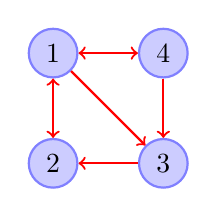
\begin{tikzpicture}[scale=.7]
            \node(A) at (0,0) [place] {2};
            \node(B) at (2,0) [place] {3};
            \node(C) at (2,2) [place] {4};
            \node(D) at (0,2) [place] {1};
            
            \draw[red,thick,<->] (A.north) -- (D.south);
            \draw[red,thick,->]  (C.south) -- (B.north);
            \draw[red,thick,->]  (D.south east) -- (B.north west);
            \draw[red,thick,<->] (D.east) -- (C.west);
            \draw[red,thick,<-]  (A.east) -- (B.west);
          \end{tikzpicture}
        \end{center}
      \end{figure}
      \pause 
      若令
      $$
      a_{ij} = \left\{
      \begin{array}{ll}
        1, & \mbox{从$i$市到$j$市有1条单向航线}\\[0.2cm]
        0, & \mbox{从$i$市到$j$市没有单向航线}
      \end{array}
      \right.
      $$ \pause 
      则该航线图可用矩阵表示为
      \begin{figure}
        \centering
        \begin{tikzpicture}
          \matrix (M) [matrix of math nodes]  { 
            \A = \\
          };
          \matrix(MM) [right=.5in of M, matrix of math nodes,nodes in empty cells,
            column sep=4ex,row sep=.5ex,ampersand replacement=\&,left delimiter=(,right delimiter=)] {
            0 \& 1 \& 1 \& 1\\
            1 \& 0 \& 0 \& 0\\
            0 \& 1 \& 0 \& 0\\
            1 \& 0 \& 1 \& 0\\
          };
          \node[above=4pt  of MM-1-1, blue]  {城市1};
          \node[above=4pt  of MM-1-2, blue]  {城市2};
          \node[above=4pt  of MM-1-3, blue]  {城市3};
          \node[above=4pt  of MM-1-4, blue]  {城市4};
          \node[left =12pt  of MM-1-1, blue]  {城市1};
          \node[left =12pt  of MM-2-1, blue]  {城市2};
          \node[left =12pt  of MM-3-1, blue]  {城市3};
          \node[left =12pt  of MM-4-1, blue]  {城市4};
        \end{tikzpicture}
      \end{figure}
    \end{exampleblock}
  \end{footnotesize}
  
\end{frame}


\begin{frame}
  \begin{footnotesize}

    \begin{exampleblock}{例3}
      设变量$x_1, x_2, \cd, x_n$与变量$y_1,y_2,\cd,y_m$满足:
      \begin{equation}\label{lt}
      \left\{
      \begin{array}{c}
        y_1  = a_{11} x_1 + a_{12} x_2 + \cd + a_{1n} x_n, \\[0.2cm]
        y_2  = a_{21} x_1 + a_{22} x_2 + \cd + a_{2n} x_n, \\[0.2cm]
             \vd \\[0.2cm]
        y_m  = a_{m1} x_1 + a_{m2} x_2 + \cd + a_{mn} x_n
      \end{array}
      \right.
      \end{equation}
      它表示一个从变量$x_1, x_2, \cd, x_n$到变量$y_1,y_2,\cd,y_m$的\red{线性变换},
      其系数$a_{ij}$构成矩阵$A=(a_{ij})_{m\times n}$。
    \end{exampleblock}
    \pause 
    \begin{itemize}
    \item  给定了线性变换(\ref{lt}),其\red{系数矩阵}也就确定。 \pause
    \item   反之,若给出一个矩阵作为线性变换的系数矩阵,则线性变换也就确定。\pause 
    \item   从这个意义上讲,线性变换与矩阵之间存在一一对应的关系。
    \end{itemize}
  \end{footnotesize}
\end{frame}

\begin{frame}
  \begin{footnotesize}
    线性变换
    $$
    \left\{
    \begin{array}{c}
      y_1 = x_1, \\[0.2cm]
      y_2 = x_2, \\[0.2cm]
      \vd \\[0.2cm]
      y_n = x_n
    \end{array}
    \right.
    $$
    称为\red{恒等变换},\pause 它对应$n$阶方阵
    $$
    \mathbf{I} = \left(
    \begin{array}{cccc}
      1    & 0    & \cd  & 0 \\
      0    & 1    & \cd  & 0 \\
      \vd  & \vd  &      & \vd \\
      0    & 0    & \cd  & 1
    \end{array}
    \right). 
    $$\pause 
    该方阵称为$n$阶\red{单位矩阵},简称\red{单位阵}。其$(i,j)$元为
    $$
    \delta_{ij} = \left \{
    \begin{array}{ll}
      1, &i=j, \\
      0, &i\ne j.
    \end{array}
    \right.  
    $$
  \end{footnotesize}
\end{frame}



\begin{frame}
  \begin{footnotesize}
    线性变换
    $$
    \left\{
    \begin{array}{c}
      y_1 = \lambda_1 x_1, \\[0.2cm]
      y_2 = \lambda_2 x_2, \\[0.2cm]
      \vd \\[0.2cm]
      y_n = \lambda_n x_n
    \end{array}
    \right.
    $$ \pause 
    它对应$n$阶方阵
    $$
    \A = \left(
    \begin{array}{cccc}
      \lambda_1& 0    & \cd  & 0 \\
      0    & \lambda_2    & \cd  & 0 \\
      \vd  & \vd  &      & \vd \\
      0    & 0    & \cd  & \lambda_n
    \end{array}
    \right)
    $$
    \pause 这种方阵称为\red{对角矩阵},简称\red{对角阵},记作
    $$
    \A = \mathrm{diag}(\lambda_1,\lambda_2,\cd,\lambda_n).
    $$
  \end{footnotesize}
\end{frame}


\begin{frame}
  \begin{footnotesize}
    矩阵
    $$
    \left(
    \begin{array}{cc}
      1 & 0 \\
      0 & 0 
    \end{array}
    \right)
    $$ \pause 
    所对应的线性变换为
    $$
    \left\{
    \begin{array}{l}
      x_1 = x, \\[0.2cm]
      y_1 = 0
    \end{array}
    \right.
    $$
    是一个投影变换。 \pause 
  \end{footnotesize}

  \begin{center}
    \begin{tikzpicture}[scale=1.0]
      %% \draw[help lines] (0,0) grid (3,3);
      \draw[<->] (0,3) node[left] {$y$} -- (0,0) -- (3,0)node[below] {$x$};
      \node[label=-150:$O$]        (P0) at (0,0) {};
      \node[label=below:$P_1$] (P1) at (2,0) {};
      \node[label=above:$P$] (P) at (2,2.5) {};
      \draw[red, thick, ->] (P0.center) -- (P1.center);
      \draw[red, thick, ->] (P0.center) -- (P.center);
      \draw[red, thick, dashed] (P.center) -- (P1.center);
    \end{tikzpicture}
  \end{center}
\end{frame}




\begin{frame}
  \begin{footnotesize}
    矩阵
    $$
    \left(
    \begin{array}{rr}
      \cos \varphi & -\sin \varphi \\
      \sin \varphi &  \cos \varphi 
    \end{array}
    \right)
    $$ \pause 
    对应的线性变换
    $$
    \left \{
    \begin{array}{l}
      x_1 = x \cos \varphi - y \sin \varphi, \\[0.2cm]
      y_1 = x \sin \varphi + y \cos \varphi, \\[0.2cm]
    \end{array}
    \right.
    $$
    设$x=r\cos \theta, y = r\sin \theta$,
    则
    $$
    \begin{array}{l}
      x_1 = r(\cos\varphi \cos\theta - \sin\varphi \sin\theta) = r\cos(\theta+\varphi), \\[0.2cm]
      y_1 = r(\sin\varphi \cos\theta + \cos\varphi \sin\theta) = r\sin(\theta+\varphi), 
    \end{array}
    $$
    \pause 
    \begin{center}
    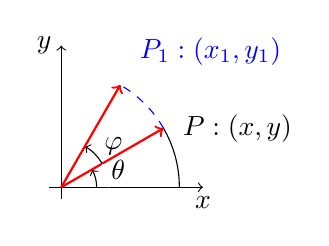
\begin{tikzpicture}[scale=1.5]
      %\draw[step=.5cm,gray,very thin] (-0.1,-0.1) grid (1.4,1.4);
      \draw[->] (-.1,0) -- (1.2,0)  node[below] {$x$};
      \draw[->] (0,-0.1) -- (0,1.2) node[left] {$y$};
      \draw[]   (1,0) arc (0:30:1) node(P)[label=right:$P:{(x,y)}$]{};
      \draw[->] (3mm,0mm) -- (3mm,0mm) arc (0:30:3mm) node(A)[label=right:$\theta$]{};
      \draw[red, thick, ->] (0,0) --  (P.center);
      \pause 
      \draw[white] (4mm,0mm) -- (4mm,0mm) arc (0:30:4mm) node(A){};
      \draw[->] (A.center) arc (30:60:4mm) node[label=right:$\varphi$]{};
      \pause
      \draw[blue, dashed]  (P) arc (30:60:1) node(P1)[label=above right:$P_1:{(x_1,y_1)}$]{};
      
      \draw[red, thick, ->] (0,0) -- (P1.center);    
    \end{tikzpicture}
  \end{center}

    这表明经过上述变换,将向量$\vec{OP}$逆时针旋转$\varphi$角得到向量$\vec{OP_1}$。
  \end{footnotesize}


\end{frame}



\begin{frame}
  \begin{overprint}
  \begin{exampleblock}{高斯消去法}
    求解线性方程组
    $$
    \left\{
    \begin{array}{rcrcrcrcrr}
      2x_1 & - & 2x_2 &   &      & + &  6x_4 & = &-2 \\[0.1cm]
      2x_1 & - &  x_2 & + & 2x_3 & + &  4x_4 & = &-2 \\[0.1cm]
      3x_1 & - &  x_2 & + & 4x_3 & + &  4x_4 & = &-3 \\[0.1cm]
      5x_1 & - & 3x_2 & + &  x_3 & + & 20x_4 & = &-2 
    \end{array}
    \right.
    $$
  \end{exampleblock}    
  \end{overprint}

  \begin{overprint}
    \only<1>{

    }    
    \only<2>{
      \textbf{解:}
      $$
      \left\{
      \begin{array}{rcrcrcrcrr}
        x_1 & - &  x_2 &   &      & + &  3x_4 & = &-1 \\[0.1cm]
        &  &  x_2 & + & 2x_3 & - &  2x_4 & = &0 \\[0.1cm]
        &  & 2x_2 & + & 4x_3 & - &  5x_4 & = &0 \\[0.1cm]
        &  & 2x_2 & + &  x_3 & + &  5x_4 & = &3 
      \end{array}
      \right.
      $$    
    } \only<3>{ 
      \textbf{解:}
      $$
      \left\{
      \begin{array}{rcrcrcrcrr}
        x_1 & - &  x_2 &   &      & + &  3x_4 & = &-1 \\[0.1cm]
        &  &  x_2 & + & 2x_3 & - &  2x_4 & = &0 \\[0.1cm]
        &  &  &  &  & - &  x_4 & = &0 \\[0.1cm]
        &  &  & - &  3x_3 & + &  9x_4 & = &3 
      \end{array}
      \right.
      $$    
    } \only<4>{
      \textbf{解:}
      $$
      \left\{
      \begin{array}{rcrcrcrcrr}
        x_1 & - &  x_2 &   &      & + &  3x_4 & = &-1 \\[0.1cm]
        &  &  x_2 & + & 2x_3 & - &  2x_4 & = &0 \\[0.1cm]
        &  &  & - &  3x_3 & + &  9x_4 & = &3 \\[0.1cm]
        &  &  &  &  & - &  x_4 & = &0 
      \end{array}
      \right.
      $$    
    } \only<5>{
      \textbf{解:}
      $$
      \left\{
      \begin{array}{rcrcrcrcrr}
        x_1 & - &  x_2 &   &      & + &  3x_4 & = &-1 \\[0.1cm]
        &  &  x_2 & + & 2x_3 & - &  2x_4 & = &0 \\[0.1cm]
        &  &  &  &  x_3 & - &  3x_4 & = &-1 \\[0.1cm]
        &  &  &  &  &  &  x_4 & = &0 
      \end{array}
      \right.
      $$    
      \pause 
      如此形状的方程组称为\red{阶梯形线性方程组}.
    } \only<6>{
      该方程组可写成矩阵形式
      \begin{figure}
        \centering
        \begin{tikzpicture}
          \matrix(M) [matrix of math nodes,nodes in empty cells,,ampersand replacement=\&,left delimiter=(,right delimiter=)]{
            A \& \& b \\
          };
          \draw[dashed] (M-1-2.north) -- (M-1-2.south);
          \matrix(M1) [right=.1in of M,matrix of math nodes]{
              = \\
          };
          \matrix(MM) [right=.1in of M1,matrix of math nodes,nodes in empty cells,
            column sep=1ex,row sep=.5ex,ampersand replacement=\&,left delimiter=(,right delimiter=)] {
            2 \& -2 \& 0 \&  6 \& \& -2\\
            2 \& -1 \& 2 \&  4 \& \& -2\\
            3 \& -1 \& 4 \&  4 \& \& -3\\
            5 \& -3 \& 1 \& 20 \& \& -2\\
          };
          \draw[dashed] (MM-1-5.north) -- (MM-4-5);
        \end{tikzpicture}
        \caption{增广矩阵}
      \end{figure}
      
    }

  \end{overprint}

\end{frame}

\begin{frame}
   \begin{figure}
        \centering
        \begin{tikzpicture}          
          \matrix(MM) [matrix of math nodes,nodes in empty cells,
            column sep=1ex,row sep=.5ex,ampersand replacement=\&,left delimiter=(,right delimiter=)] {
            2 \& -2 \& 0 \&  6 \& \& -2\\
            2 \& -1 \& 2 \&  4 \& \& -2\\
            3 \& -1 \& 4 \&  4 \& \& -3\\
            5 \& -3 \& 1 \& 20 \& \& -2\\
          };
          \draw[dashed] (MM-1-5.north) -- (MM-4-5);
        \end{tikzpicture}
        \pause 
        \begin{tikzpicture}
          \matrix (M) [matrix of math nodes]  { 
            \xlongequal[]{r_1 \times \frac12} \\
          };
          \pause 
          \matrix(MM) [right=.1in of M,matrix of math nodes,nodes in empty cells,
            column sep=1ex,row sep=.5ex,ampersand replacement=\&,left delimiter=(,right delimiter=)] {
            1 \& -1 \& 0 \&  3 \& \& -1\\
            2 \& -1 \& 2 \&  4 \& \& -2\\
            3 \& -1 \& 4 \&  4 \& \& -3\\
            5 \& -3 \& 1 \& 20 \& \& -2\\
          };
          \draw[dashed] (MM-1-5.north) -- (MM-4-5);
        \end{tikzpicture}

        \pause 
        \begin{tikzpicture}
          \matrix (M) [matrix of math nodes]  { 
            \xlongequal[
            r_3+(-3)\times r_1,~ 
            r_4+(-5)\times r_1]{r_2+(-2)\times r_1} \\
          };
          \pause 
          \matrix(MM) [right=.1in of M,matrix of math nodes,nodes in empty cells,
            column sep=1ex,row sep=.5ex,ampersand replacement=\&,left delimiter=(,right delimiter=)] {
            1 \& -1 \& 0 \&  3 \& \& -1\\
            0 \&  1 \& 2 \& -2 \& \&  0\\
            0 \&  0 \& 0 \& -1 \& \&  0\\
            0 \&  0 \&-3 \&  9 \& \&  3\\
          };
          \draw[dashed] (MM-1-5.north) -- (MM-4-5);
        \end{tikzpicture}
      \end{figure}
\end{frame}


\begin{frame}
   \begin{figure}
        \centering
        
        \begin{tikzpicture}
          \matrix(MM) [matrix of math nodes,nodes in empty cells,
            column sep=1ex,row sep=.5ex,ampersand replacement=\&,left delimiter=(,right delimiter=)] {
            1 \& -1 \& 0 \&  3 \& \& -1\\
            0 \&  1 \& 2 \& -2 \& \&  0\\
            0 \&  0 \& 0 \& -1 \& \&  0\\
            0 \&  0 \&-3 \&  9 \& \&  3\\
          };
          \draw[dashed] (MM-1-5.north) -- (MM-4-5);
        \end{tikzpicture}
        \pause 
        \begin{tikzpicture}
          \matrix (M) [matrix of math nodes]  { 
            \xlongequal[]{r_3 \leftrightarrow r_4} \\
          };

          \pause 
          \matrix(MM) [right=.1in of M,matrix of math nodes,nodes in empty cells,
            column sep=1ex,row sep=.5ex,ampersand replacement=\&,left delimiter=(,right delimiter=)] {
            1 \& -1 \& 0 \&  3 \& \& -1\\
            0 \&  1 \& 2 \& -2 \& \&  0\\
            0 \&  0 \&-3 \&  9 \& \&  3\\
            0 \&  0 \& 0 \& -1 \& \&  0\\
          };
          \draw[dashed] (MM-1-5.north) -- (MM-4-5);
        \end{tikzpicture}

        \pause 
        \begin{tikzpicture}
          \matrix (M) [matrix of math nodes]  { 
            \xlongequal[]{r_3 \div (-3)} \\
          };
          \matrix(MM) [right=.1in of M,matrix of math nodes,nodes in empty cells,
            column sep=1ex,row sep=.5ex,ampersand replacement=\&,left delimiter=(,right delimiter=)] {
            1 \& -1 \& 0 \&  3 \& \& -1\\
            0 \&  1 \& 2 \& -2 \& \&  0\\
            0 \&  0 \& 1 \& -3 \& \& -1\\
            0 \&  0 \& 0 \&  1 \& \&  0\\
          };
          \draw[dashed] (MM-1-5.north) -- (MM-4-5);
        \end{tikzpicture}
      \end{figure}
\end{frame}


\begin{frame}
  \begin{overprint}
    \begin{exampleblock}{例}
      求解线性方程组
      $$
      \left\{
      \begin{array}{rcrcrcrcrcrr}
         x_1 & - &  x_2 & - &  x_3 &   &       & + & 3x_5 & = &-1 \\[0.1cm]
        2x_1 & - & 2x_2 & - &  x_3 & + &  2x_4 & + & 4x_5 & = &-2 \\[0.1cm]
        3x_1 & - & 3x_2 & - &  x_3 & + &  4x_4 & + & 5x_5 & = &-3 \\[0.1cm]
         x_1 & - &  x_2 & + &  x_3 & + &   x_4 & + & 8x_5 & = & 2 
      \end{array}
      \right.
      $$
    \end{exampleblock}    
  \end{overprint}
  \pause 
  \begin{overprint}
    其增广矩阵为
    \begin{figure}
      \centering
      
      \begin{tikzpicture}
        \matrix(MM) [matrix of math nodes,nodes in empty cells,
          column sep=1ex,row sep=.5ex,ampersand replacement=\&,left delimiter=(,right delimiter=)] {
          1 \& -1 \& -1 \&  0 \& 3 \& \& -1\\
          2 \& -2 \& -1 \&  2 \& 4 \& \& -2\\
          3 \& -3 \& -1 \&  4 \& 5 \& \& -3\\
          1 \& -1 \&  1 \&  1 \& 8 \& \&  2\\
        };
        \draw[dashed] (MM-1-6.north) -- (MM-4-6);
      \end{tikzpicture}
      
    \end{figure}

  \end{overprint}
  \end{frame}


\begin{frame}
  \begin{footnotesize}
    \begin{figure}
      \centering
      \begin{tikzpicture}
        \matrix(M1) [matrix of math nodes,nodes in empty cells,
          column sep=1ex,row sep=.5ex,ampersand replacement=\&,left delimiter=(,right delimiter=)] {
          1 \& -1 \& -1 \&  0 \& 3 \& \& -1\\
          2 \& -2 \& -1 \&  2 \& 4 \& \& -2\\
          3 \& -3 \& -1 \&  4 \& 5 \& \& -3\\
          1 \& -1 \&  1 \&  1 \& 8 \& \&  2\\
        };
        \draw[dashed] (M1-1-6.north) -- (M1-4-6);
        \pause
        \matrix (M2) [right=.1in of M1,matrix of math nodes]  { 
          \xlongequal[r_3+(-3)\times r_1 \atop r_4+(-1)\times r_1]{r_2+(-2)\times r_1}\\
        };
        \pause
        \matrix(MM) [right=.1in of M2,matrix of math nodes,nodes in empty cells,
          column sep=1ex,row sep=.5ex,ampersand replacement=\&,left delimiter=(,right delimiter=)] {
          1 \& -1 \& -1 \&  0 \& 3 \& \& -1\\
          0 \&  0 \&  1 \&  2 \&-2 \& \&  0\\
          0 \&  0 \&  2 \&  4 \&-4 \& \&  0\\
          0 \&  0 \&  2 \&  1 \& 5 \& \&  3\\
        };
        \draw[dashed] (MM-1-6.north) -- (MM-4-6);
      \end{tikzpicture}
      \pause
      \begin{tikzpicture}
        \matrix (M2) [,matrix of math nodes]  { 
          \xlongequal[r_3+(-2)\times r_2]{r_3+(-2)\times r_2}\\
        };\pause
        \matrix(MM) [right=.1in of M2,matrix of math nodes,nodes in empty cells,
          column sep=1ex,row sep=.5ex,ampersand replacement=\&,left delimiter=(,right delimiter=)] {
          1 \& -1 \& -1 \&  0 \& 3 \& \& -1\\
          0 \&  0 \&  1 \&  2 \&-2 \& \&  0\\
          0 \&  0 \&  0 \&  0 \& 0 \& \&  0\\
          0 \&  0 \&  0 \& -3 \& 9 \& \&  3\\
        };
        \draw[dashed] (MM-1-6.north) -- (MM-4-6);
      \end{tikzpicture}
      \pause
      \begin{tikzpicture}
        \matrix (M2) [,matrix of math nodes]  { 
          \xlongequal[r_3 \leftrightarrow r_4]{r_4\div(-3)}\\
        };\pause
        \matrix(MM) [right=.1in of M2,matrix of math nodes,nodes in empty cells,
          column sep=1ex,row sep=.5ex,ampersand replacement=\&,left delimiter=(,right delimiter=)] {
          1 \& -1 \& -1 \&  0 \& 3 \& \& -1\\
          0 \&  0 \&  1 \&  2 \&-2 \& \&  0\\
          0 \&  0 \&  0 \&  1 \& -3 \& \& -1\\
          0 \&  0 \&  0 \&  0 \& 0 \& \&  0\\
        };
        \draw[dashed] (MM-1-6.north) -- (MM-4-6);
      \end{tikzpicture}
      
      
    \end{figure}
  \end{footnotesize}
\end{frame}


\begin{frame}
  \begin{footnotesize}
    \begin{figure}
      \centering
      \begin{tikzpicture}
        \matrix(MM) [matrix of math nodes,nodes in empty cells,
          column sep=1ex,row sep=.5ex,ampersand replacement=\&,left delimiter=(,right delimiter=)] {
          1 \& -1 \& -1 \&  0 \& 3 \& \& -1\\
          0 \&  0 \&  1 \&  2 \&-2 \& \&  0\\
          0 \&  0 \&  0 \&  1 \& -3 \& \& -1\\
          0 \&  0 \&  0 \&  0 \& 0 \& \&  0\\
        };
        \draw[dashed] (MM-1-6.north) -- (MM-4-6);
        \matrix (M2) [right=.1in of MM,matrix of math nodes]  { 
          \xlongequal[]{r_2+(-2)\times r_3}\\
        };\pause
        \matrix(MM) [right=.1in of M2,matrix of math nodes,nodes in empty cells,
          column sep=1ex,row sep=.5ex,ampersand replacement=\&,left delimiter=(,right delimiter=)] {
          1 \& -1 \& -1 \&  0 \& 3 \& \& -1\\
          0 \&  0 \&  1 \&  0 \& 4 \& \&  2\\
          0 \&  0 \&  0 \&  1 \& -3 \& \& -1\\
          0 \&  0 \&  0 \&  0 \& 0 \& \&  0\\
        };
        \draw[dashed] (MM-1-6.north) -- (MM-4-6);
      \end{tikzpicture}

      \begin{tikzpicture}
        \matrix (M2) [matrix of math nodes]  { 
          \xlongequal[]{r_1+ r_2}\\
        };\pause
        \matrix(MM) [right=.1in of M2,matrix of math nodes,nodes in empty cells,
          column sep=1ex,row sep=.5ex,ampersand replacement=\&,left delimiter=(,right delimiter=)] {
          1 \& -1 \& -1 \&  0 \& 7 \& \&  1\\
          0 \&  0 \&  1 \&  0 \& 4 \& \&  2\\
          0 \&  0 \&  0 \&  1 \& 3 \& \& -1\\
          0 \&  0 \&  0 \&  0 \& 0 \& \&  0\\
        };
        \draw[dashed] (MM-1-6.north) -- (MM-4-6);
      \end{tikzpicture}
    \end{figure}
    \pause 
    该矩阵称为\red{行简化阶梯矩阵},对应的线性方程组为
    $$
    \left\{
    \begin{array}{rcrcrcrcrcrr}
       x_1 & - &  x_2 &   &      &   &       & + & 7x_5 & = & 1 \\[0.1cm]
           &   &     &   &  x_3 &   &     & + & 4x_5 & = & 2 \\[0.1cm]
           &   &   &   &    &   &   x_4 & - & 3x_5 & = &-1
    \end{array}
    \right.
    $$
  \end{footnotesize}
\end{frame}

\begin{frame}
  \begin{footnotesize}
    $$
    \left\{
    \begin{array}{rcrcrcrcrcrr}
      x_1 & - &  x_2 &   &      &   &       & + & 7x_5 & = & 1 \\[0.1cm]
      &   &     &   &  x_3 &   &     & + & 4x_5 & = & 2 \\[0.1cm]
      &   &   &   &    &   &   x_4 & - & 3x_5 & = &-1
    \end{array}
    \right.
    $$
    \pause
    \begin{block}{注}
      该方程组有$5$个未知量,其中$x_1,x_3,x_4$为\red{基本未知量},$x_2,x_5$为\red{自由未知量}。
    \end{block}
    \pause 
    任取$x_2=k_1, x_5=k_2$,可得线性方程组的全部解
    $$
    \left\{
    \begin{array}{ccl}
      x_1 &=& 1+k_1-7k_2, \\[0.1cm]      
      x_2 &=& k_1, \\[0.1cm]
      x_3 &=& 2-4k_2, \\[0.1cm]
      x_4 &=& -1+3k_2,\\[0.1cm]
      x_5 &=& k_2.
    \end{array}
    \right.
    $$
    
  \end{footnotesize}
\end{frame}


\begin{frame}
  \begin{footnotesize}
    \begin{exampleblock}{例}
      解线性方程组
      $$
      \left\{
      \begin{array}{rcrcrcr}
         x_1 & + & x_2 & + &  x_3 & = & 1, \\[0.1cm]
         x_1 & + &2x_2 & - & 5x_3 & = & 2, \\[0.1cm]
        2x_1 & + &3x_2 & - & 4x_3 & = & 5.
      \end{array}
      \right.
      $$
    \end{exampleblock}


    \begin{figure}
      \begin{tikzpicture}
        
        \matrix(MM) [matrix of math nodes,nodes in empty cells,
          column sep=1ex,row sep=.5ex,ampersand replacement=\&,left delimiter=(,right delimiter=)] {
          1 \&  1 \&  1 \& \&  1\\
          1 \&  2 \& -5 \& \&  2\\
          2 \&  3 \& -4 \& \&  5\\
        };
        \draw[dashed] (MM-1-4.north) -- (MM-3-4);
        \pause
        \matrix (M2) [right=.1in of MM,matrix of math nodes]  { 
          \xlongequal[r_3+ (-2)\times r_1]{r_2+ (-1)\times r_1}\\
        };\pause

        \matrix(MM) [right=.1in of M2,matrix of math nodes,nodes in empty cells,
          column sep=1ex,row sep=.5ex,ampersand replacement=\&,left delimiter=(,right delimiter=)] {
          1 \&  1 \&  1 \& \&  1\\
          0 \&  1 \& -6 \& \&  1\\
          0 \&  1 \& -6 \& \&  3\\
        };
        \draw[dashed] (MM-1-4.north) -- (MM-3-4);
        
      \end{tikzpicture}

      \pause
      \begin{tikzpicture}
        \matrix (M2) [right=.1in of MM,matrix of math nodes]  { 
          \xlongequal[]{r_3+ (-1)\times r_2}\\
        };\pause

        \matrix(MM) [right=.1in of M2,matrix of math nodes,nodes in empty cells,
          column sep=1ex,row sep=.5ex,ampersand replacement=\&,left delimiter=(,right delimiter=)] {
          1 \&  1 \&  1 \& \&  1\\
          0 \&  1 \& -6 \& \&  1\\
          0 \&  0 \&  0 \& \&  2\\
        };
        \draw[dashed] (MM-1-4.north) -- (MM-3-4);
        
      \end{tikzpicture}
    \end{figure}
    \pause
    由第三行可以看出,该线性方程组无解。
  \end{footnotesize}
\end{frame}

\begin{frame}
  \begin{itemize}
  \item 含有矛盾方程而无解的方程组称为\red{不相容方程组} \\[0.2cm]
  \item 有解的方程组称为\red{相容方程组}  \\[0.2cm]
  \item \red{多余方程}
  \end{itemize}
\end{frame}



\begin{frame}
  \begin{footnotesize}
    对于一般的线性方程组
    $$
    \left\{
    \begin{array}{c}
      a_{11}x_1 + a_{12}x_2 + \cd + a_{1n}x_n = b_1\\[0.2cm]
      a_{21}x_1 + a_{22}x_2 + \cd + a_{2n}x_n = b_2\\[0.2cm]
      \vd\\[0.2cm]
      a_{m1}x_1 + a_{m2}x_2 + \cd + a_{mn}x_n = b_m
    \end{array}
    \right.
    $$
    增广矩阵为
    \begin{figure}
      \begin{tikzpicture}
        \matrix(MM) [matrix of math nodes,nodes in empty cells,
          column sep=1ex,row sep=.5ex,ampersand replacement=\&,left delimiter=(,right delimiter=)] {
          a_{11} \&  a_{12} \&  \cd \& a_{1n} \& \&  b_1\\
          a_{21} \&  a_{22} \&  \cd \& a_{2n} \& \&  b_2\\
          \vd   \&  \vd   \&      \&  \vd  \& \& \vd \\
          a_{m1} \&  a_{m2} \&  \cd \& a_{mn} \& \&  b_m\\
        };
        \draw[dashed] (MM-1-5.north) -- (MM-4-5);
        
      \end{tikzpicture}
      
    \end{figure}
  \end{footnotesize}
\end{frame}


\begin{frame}
  \begin{footnotesize}
    \begin{figure}
      \begin{tikzpicture}
        \matrix(MM) [matrix of math nodes,nodes in empty cells,
          column sep=0.6ex,row sep=.5ex,ampersand replacement=\&,left delimiter=(,right delimiter=)] {
          a_{11} \&  a_{12} \&  \cd \& a_{1n} \& \&  b_1\\
          a_{21} \&  a_{22} \&  \cd \& a_{2n} \& \&  b_2\\
          \vd   \&  \vd   \&      \&  \vd  \& \& \vd \\
          a_{m1} \&  a_{m2} \&  \cd \& a_{mn} \& \&  b_m\\
        };
        \draw[dashed] (MM-1-5.north) -- (MM-4-5);
        \pause
        \matrix (M2) [right=.05in of MM,matrix of math nodes]  { 
          \Rightarrow\\
        };
        \pause
        \matrix(MM) [right=.05in of M2,matrix of math nodes,nodes in empty cells,
          column sep=0.6ex,row sep=.5ex,ampersand replacement=\&,left delimiter=(,right delimiter=)] {
          c_1 \&   0 \& \cd \&  0 \& c_{1,r+1} \& \cd \& c_{1n} \& \& d_1\\
          0   \& c_2 \& \cd \&  0 \& c_{2,r+1} \& \cd \& c_{2n} \& \& d_2\\
          \vd \& \vd \& \dd \&\vd \& \vd     \&     \& \vd   \& \& \vd\\
          0   \&  0  \& \cd \& c_{rr} \& c_{r,r+1} \& \cd \& c_{rn} \& \& d_r\\
          0   \&  0  \& \cd \& 0 \& 0 \& \cd \& 0 \&  \& d_{r+1}\\
          0   \&  0  \& \cd \& 0 \& 0 \& \cd \& 0 \&  \& 0\\          
          \vd \& \vd \& \dd \&\vd \& \vd     \&     \& \vd   \& \& \vd\\
          0   \&  0  \& \cd \& 0 \& 0 \& \cd \& 0 \&  \& 0\\
        };
        \draw[dashed] (MM-1-8.north) -- (MM-8-8);
        \filldraw[opacity=0.5,red!50] (MM-5-9) circle (0.3cm);
      \end{tikzpicture}      
    \end{figure}
    其中$c_{ii}=1~(i=1,2,\cd,r)$.
  \end{footnotesize}
\end{frame}

\begin{frame}
  \begin{footnotesize}
    
    \begin{itemize}
    \item[1] 线性方程组有解$ \Leftrightarrow \red{d_{r+1}=0}$;
    \item[2] 在有解的情况下:
      \begin{itemize}
      \item 当$r=n$时,有唯一解$x_1=d_1,~x_2=d_2,~\cd,~x_n=d_n$;
      \item 当$r<n$时,有无穷多解
        $$
        \left\{
        \begin{array}{ccl}
          x_1 &=& d_1 - c_{1,r+1}k_1 - \cd - c_{1n}k_{n-r}, \\[0.1cm]
          x_2 &=& d_2 - c_{2,r+1}k_1 - \cd - c_{2n}k_{n-r}, \\[0.1cm]
          \vd & & \vd \\[0.1cm]
          x_r &=& d_r - c_{r,r+1}k_1 - \cd - c_{rn}k_{n-r}, \\[0.1cm]
          x_{r+1} &=& k_1, \\[0.1cm]
          \vd && \vd \\[0.1cm]
          x_{n} &=& k_{n-r}.
        \end{array}
        \right.
        $$
      \end{itemize}
    \end{itemize}     
  \end{footnotesize}
\end{frame}
